\chapter{Introduction}

The main focus of this study was to look at the gravitational collapse of a scalar field in the light of swampland distance conjecture. In the following sections we will briefly touch upon these topics and give suitable references for further explorations.

\section{Gravitational collapse of scalar fields}


Critical collapse of scalar fields in gravitation is a well studied phenomenon \citep{Gundlach:2007gc}, and there are many interesting results mostly based on the numerical simulations.
Gravitational collapse and the numerical methods used to study it will be described in detail in a later chapter. Here we will just mention one result that will be required to put things that we are going to discuss into perspective.
Assume that the initial configuration of the scalar field is described by a function with n adjustable parameters that we are free to choose. Then for each one of those n parameters there will be a corresponding threshold, crossing which will lead to the formation of a black hole.

For example, if the initial scalar field configuration is a gaussian with fixed mean and variance, then there will a critical value of the amplitude (let’s call it $A_0$ ) above which black hole formation will take place. Although, if we keep the amplitude (A) below $A_0$ then the scalar field will disperse to infinity. The same holds true for the
mean and the variance.

Another important observation is that even if the initial value of the amplitude A and the critical value $A_0$ are both much smaller than 1 (in natural units), field movement near the origin for $A >= A_0$ can still be of the $O(1)$ (again in natural unit scale) in the scalar field space. We will expand upon and give examples of this in later chapters.
For this chapter it is enough to remember that in general relativity scalar fields can move $O(1)$ distance in the scalar field space, starting from much smaller values.

\section{Swampland conditions}
Before we can appreciate what are swampland conditions we need to understand a little bit about effective field theories and the role that they play in Physics.

\subsection{Effective field theories}
Physical phenomenon occurs at various scales, sometimes we are only interested in the results at a particular scale. For example, if we are interested in the collision of two slow moving bodies then Newtonian mechanics is more than enough, we do not need to consider Relativistic mechanics. The scale of interest in this case is the speed of the bodies and for speeds much smaller than the speed of light we can
consider Newtonian mechanics as an "effective theory" of Relativistic mechanics.

Such theories in the context of QFT are known as "effective field theories". Roughly speaking we can set the parameters much smaller and larger than the physical
quantities we are interested in to zero and infinity respectively. After that, any effects due to these approximations can be included as small perturbations.

A prime example of an effective field theory is Fermi theory of weak interactions. It was phenomenally constructed by Fermi as a modification to QED which accounted for the neutron decay. Now that we have the Standard model, we understand that the Fermi theory is an effective field theory valid for energy scales much smaller than the mass of W boson.

Effective theories are ubiquitous in Physics, whether it is for the ease of calculations (it is not an efficient use of time to track motion of a football using GR) or because they are a part of how Physics progresses (nobody could have constructed the Standard model lagrangian without the insights gained from all the effective field theories).
If we have a more "complete" theory, then it is a comparatively easy matter to generate effective theories as per our needs. At this point one can ask a question, can all field theories be extended into more general and complete theories?
The exact question that we are interested in is what kind of effective field theories can be completed into quantum gravity in the high energy or UV regime? This is the question that swampland conditions try to answer.


\subsection{The landscape and the swampland}
A lot of low energy effective field theories, each corresponding to a different vacuum, can be constructed from the string theory. The collection of such effective field theories constructed from the string theory is called the landscape. At the same time, there are a lot of other low energy self-consistent theories that do not come from the string theory, the collection of all such theories is called the swampland.

\begin{figure}[hbt!]
    \centering
    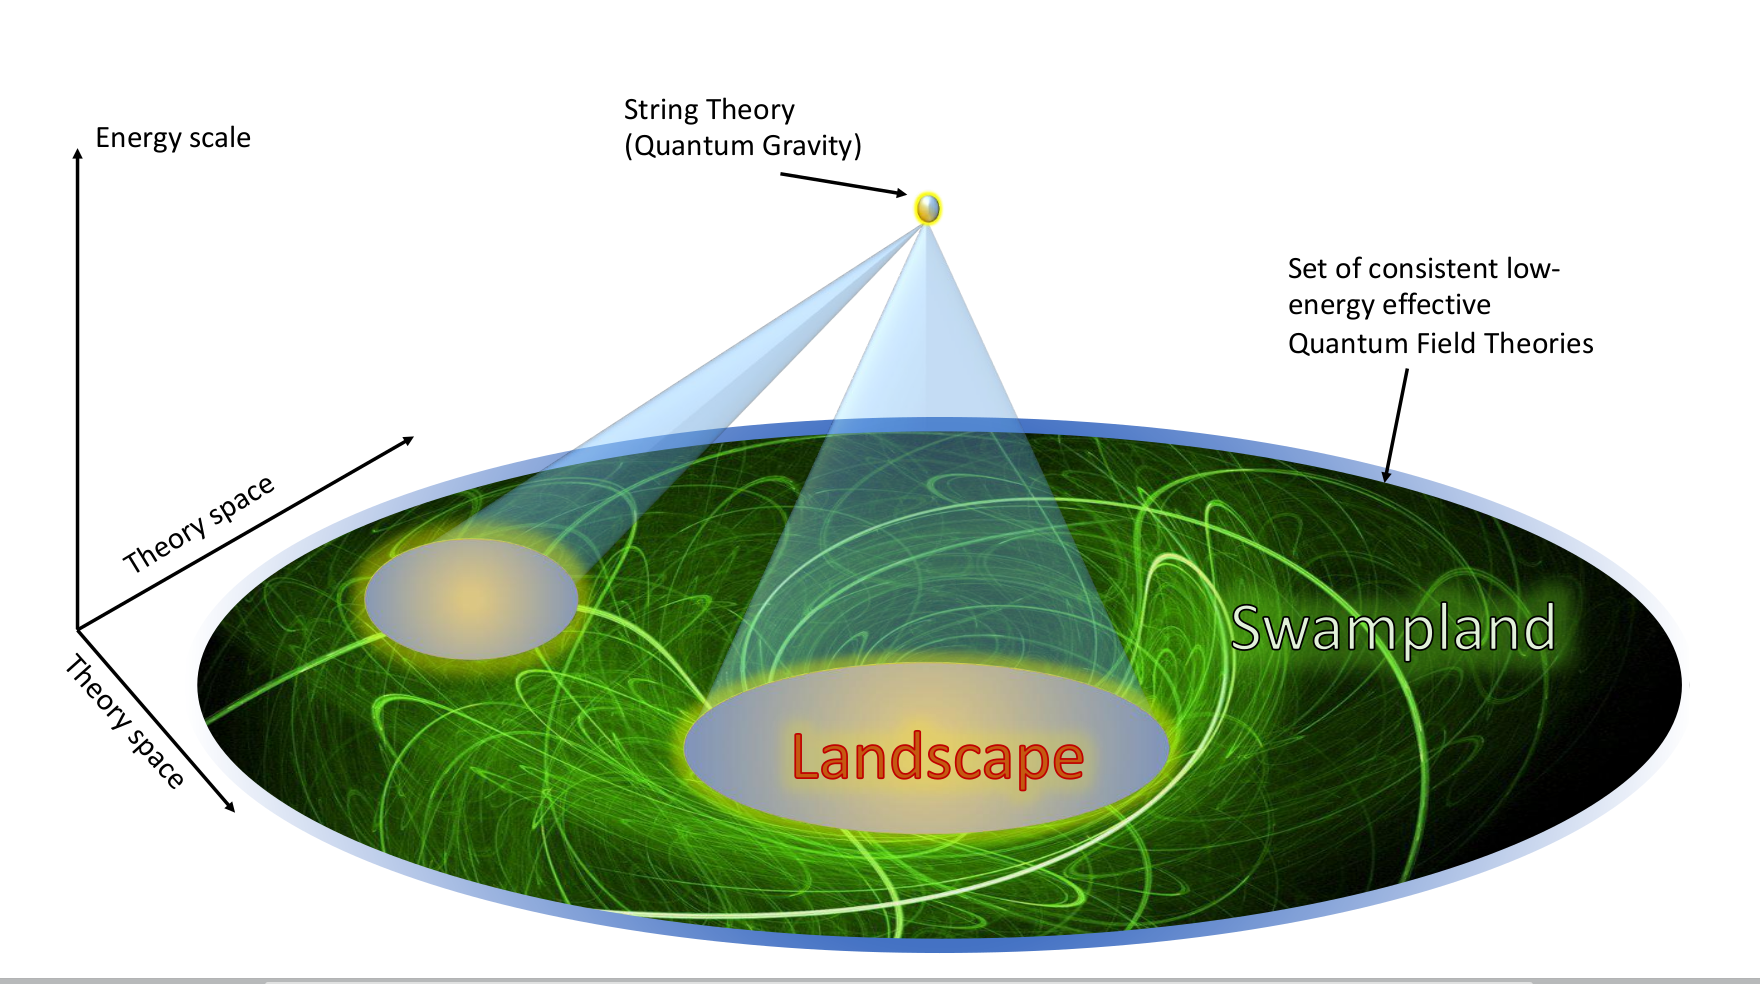
\includegraphics[width=\textwidth]{images/swampland.png}
    \caption{Landscape and the swampland. Y-axis represents energy scale. Effective field theories in the landscape can be UV completed to string theory. Taken from \citep{Palti:2019pca}}
    \label{swampland and landscape}
\end{figure}

In other words, we can complete a low energy theory from the landscape into a UV theory of quantum gravity. But, trying to UV complete a theory form the swampland into a theory of quantum gravity leads to inconsistencies. The idea of the landscape and the swampland is pictorially shown in the figure 1.1.

\subsection{Swampland distance conjecture}
Whether an effective field theory exists in the swampland or the landscape is the question that swampland conditions try to answer. Although, there are quite a few of these conditions most of them do not have any formal proof from microscopic physics perspective and are thus treated as conjectures. The confidence that we have in these conjectures mostly comes from the observations based on the few known vacua of the string theory and quantum gravity arguments \citep{Palti:2019pca} \citep{Brennan:2017rbf}.


One thing worth mentioning is that the swampland conjectures are defined completely in terms of the low energy effective field theory without any reference to its ultraviolet origin, which implies that the effective field theory has some knowledge about its ultraviolet origin. This is a little unsettling from the renormalization group point of view, which strongly suggests that there is a scale separation in Physics,i.e. low energy theories should not have any knowledge about their ultraviolet counterpart.

One of these conjectures is the swampland distance conjecture (SDC), which states that an effective field theory that has gravity and scalar fields cannot be reliable in the regions where the scalar field moves beyond an $O(1)$ range.
But, we know that $O(1)$ field movement is observed in the case of black hole formation due to the scalar field collapse, as mentioned in the section 1.1. This tension between the SDC and gravitational collapse of a scalar field in general
relativity is what we will be exploring in this thesis.